
\begin{figure}
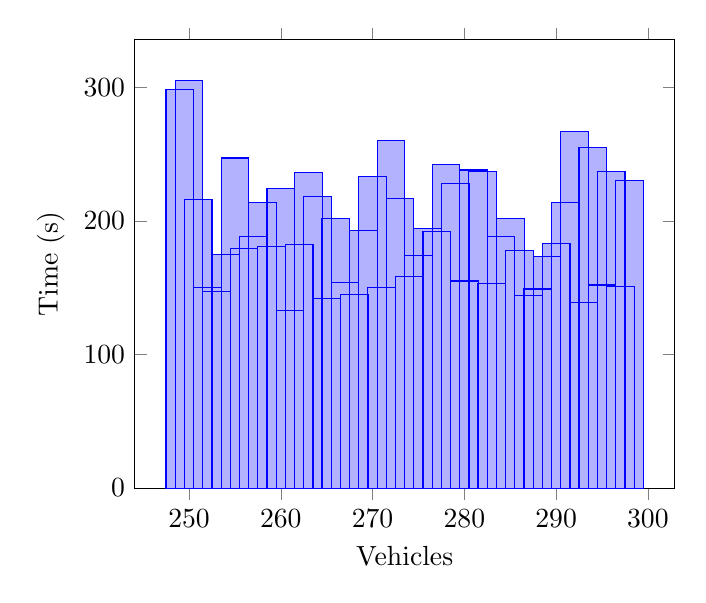
\begin{tikzpicture}
\begin{axis}[
legend style={anchor=west},
xlabel=Vehicles,
ylabel=Time (s),
ymin=0,
ybar,
]
\addplot coordinates {
(298, 230)
(296, 237)
(297, 151)
(294, 255)
(295, 152)
(292, 267)
(293, 139)
(290, 183)
(291, 214)
(270, 233)
(271, 150)
(272, 260)
(273, 217)
(274, 158)
(275, 174)
(276, 194)
(277, 192)
(278, 242)
(279, 228)
(249, 298)
(252, 150)
(258, 214)
(259, 181)
(250, 305)
(251, 216)
(256, 179)
(257, 188)
(254, 175)
(261, 133)
(289, 173)
(288, 149)
(281, 238)
(280, 155)
(282, 237)
(285, 202)
(284, 188)
(287, 144)
(286, 178)
(263, 236)
(262, 182)
(260, 224)
(267, 154)
(266, 202)
(265, 142)
(264, 218)
(269, 193)
(268, 145)
(253, 147)
(283, 153)
(255, 247)
};

\end{axis}
\end{tikzpicture}
\label{tik:time:0:91}
\caption{0 percent diving with GSC on route $91$}
\end{figure}
